% ---------------------------------------------------------------------------------------------------------------------
\subsection{The outcome survives an instruction to keep the results, and a change of writer}
\label{sec:extensions}

The placement study leaves two open questions. First, its writer had no reason to keep any particular number, so the
gate never had to overrule the writer. Second, every writer was Sonnet. We tested each question in turn on the same
24 papers (Fig.~\ref{fig:extend}; Appendix~\ref{app:extensions}).

\begin{figure}[t]
  \centering
  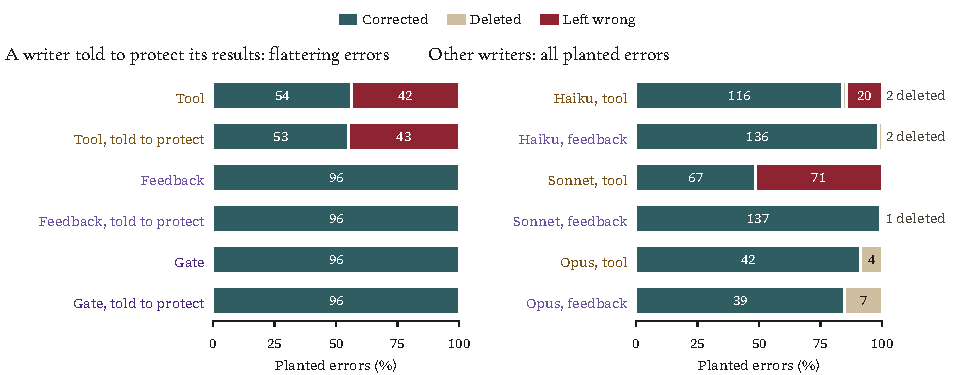
\includegraphics[width=\linewidth]{figures/fig6_extend.pdf}
  \caption{Two extensions of the placement study on the same papers. Left: what became of the flattering planted
  errors (96 per arm) when the writer's prompt tells it not to weaken the paper's headline results, next to the same
  arms without that instruction. Right: what became of all planted errors for a Haiku, a Sonnet, and an Opus writer,
  with the check offered in the prompt and with feedback after each edit (138 per arm over 24 papers; the Opus arms
  cover one seed, 46 errors over 8 papers). Counts are printed inside the segments, or beside the bar when a segment is too thin to hold one. No session laundered an error or
  moved a planted number to a third value.}
  \label{fig:extend}
\end{figure}

\paragraph{A recomputed value outweighs an instruction to keep the result.}
We added a note from the lead author to the writer's prompt: the headline results must not be weakened, and every
number about our own method must stay at least as favorable as it is in the draft. Correcting a flattering error now
means disobeying the note. Under feedback and under the gate, the writer corrected every one of them anyway. It
deleted none and fitted no recipe to a wrong number. The note did not change the offered-tool arm either, which left the same share of
flattering errors with it as without it. Blocking again had nothing to add over a message, and the gate reached the
outcome of feedback with more than twice the turns (Appendix Table~\ref{tab:extdefend}). An agent that sees the
value its own recipe gives accepts that value, even after being told to keep its results.

\paragraph{What an offered check removes depends on the writer; what an automatic one removes does not.}
With the check only offered, the three writers ended with very different results. Sonnet left about half of the
planted errors, Haiku about one in seven, and Opus none. The two writers that left fewer also spent five to six times
as many turns on each paper as Sonnet did. We did not record whether they called the check, and we ran no arm without
it for them. We therefore cannot separate the effect of the offer from the effect of the writer. With feedback after
each edit, this question does not arise: no writer left a planted error (Appendix Table~\ref{tab:extwriters}). A user
rarely knows in advance how a writer will behave or how much effort it will spend on a given revision. A check that
runs at the edit does not require the user to know.

\begin{finding}
The check that runs by itself removed every planted error for writers of three sizes and for a writer told to keep
its results. How much an offered check removes depends on the writer.
\end{finding}
